% !TeX spellcheck = en_US
\section{Design of a Novel MBS}
\label{sec:522_Liviu}
The proposed adaptation between different video upload protocols results in significant costs, as, e.g., the receiver side needs to maintain all protocol stacks in an active state.
Derived from the previous study, a novel, adaptive \ac{MBS} called \ac{LiViU} is proposed.
\subsection{Features of LiViU}
\ac{LiViU} relies on a set of features which are derived from the discussed application scenarios and the conducted simulative study:
\begin{DesignPrinciples}
\item Support for multiple streaming scenarios.
\item Support for content and mechanism adaptation.
\item Leveraging \ac{UDP} as a transport layer protocol.
\item Support for auxiliary data transport.
\item Encapsulation of transmission functionality. 
\end{DesignPrinciples} 

\ac{LiViU} supports remote, in situ and hybrid streaming scenarios and aims for reliable and efficient video collection. 
Mechanisms have to be proposed that aim at (1) a high bit rate but rather high delay - e.g., several seconds -  for remote streaming as well as (2) low-delay - e.g., milliseconds - and rather low bit rates for in situ streaming.
\ac{LiViU} must be capable to support receivers of both remote and in situ streaming at the same time.

\ac{LiViU} allows \emph{adaptations} of both the \emph{content} and the \emph{scheduling mechanisms}.
\emph{Content adaptation} should be realized using adaptive video streaming.
Each device produces multiple representations in parallel.
Adaptation of the networks addresses the usage of scheduling mechanisms, i.e., either push- or pull-based delivery.
The different scheduling schemes have shown varying benefits depending  on multimedia application requirements and environmental conditions.
Whereas push-based delivery shows a minimal delay in delivery and generates reduced overhead, multimedia applications such as video composition benefit from a centrally controlled, pull-based media upload.
In relation to the scenario, remote, in situ, or hybrid streaming, the management functions of \ac{LiViU} have to adapt as well.

As a result of the superior performance for live streaming scenarios, \ac{LiViU} uses the unreliable \emph{\ac{UDP}} in the transport layer and compensates its weaknesses by additional application layer mechanisms.
\ac{LiViU} is message-oriented.
It copes with the degraded reliability by ensuring the processing of messages in the correct order and integrates error compensation mechanisms.

The protocol shall be able to transport \emph{media streams}, as well as \emph{auxiliary data}, which can be monitoring data such as performance metrics as well as auxiliary sensor data such as locations, accelerometer or other device sensors.
Auxiliary data can be leveraged by the multimedia application, which consumes the media streams and is essential if the \ac{PaSC} (see Chapter~\ref{chapter:550_scalable_quality_assessment}) is used.
The protocols shall be used to transport both media, i.e., audio and video, and auxiliary sensor data.

An overview of the architecture of \ac{LiViU} is given in Figure~\ref{fig:522_architectureliviu}.
It depicts the concepts of \emph{media management}, which addresses all video and auxiliary-data-relevant functionality, as well as the \emph{transmission} functionality, which addresses concepts introduced in \ac{LiViU} to send and receive data.
The yellow boxes depict modules required for the remote (as well as any other) scenario, the gray boxes indicate functionality needed for in situ streaming, which is discussed in Section~\ref{sec:534_AdhocLiviu}.
\begin{figure}[tbh]
\centering
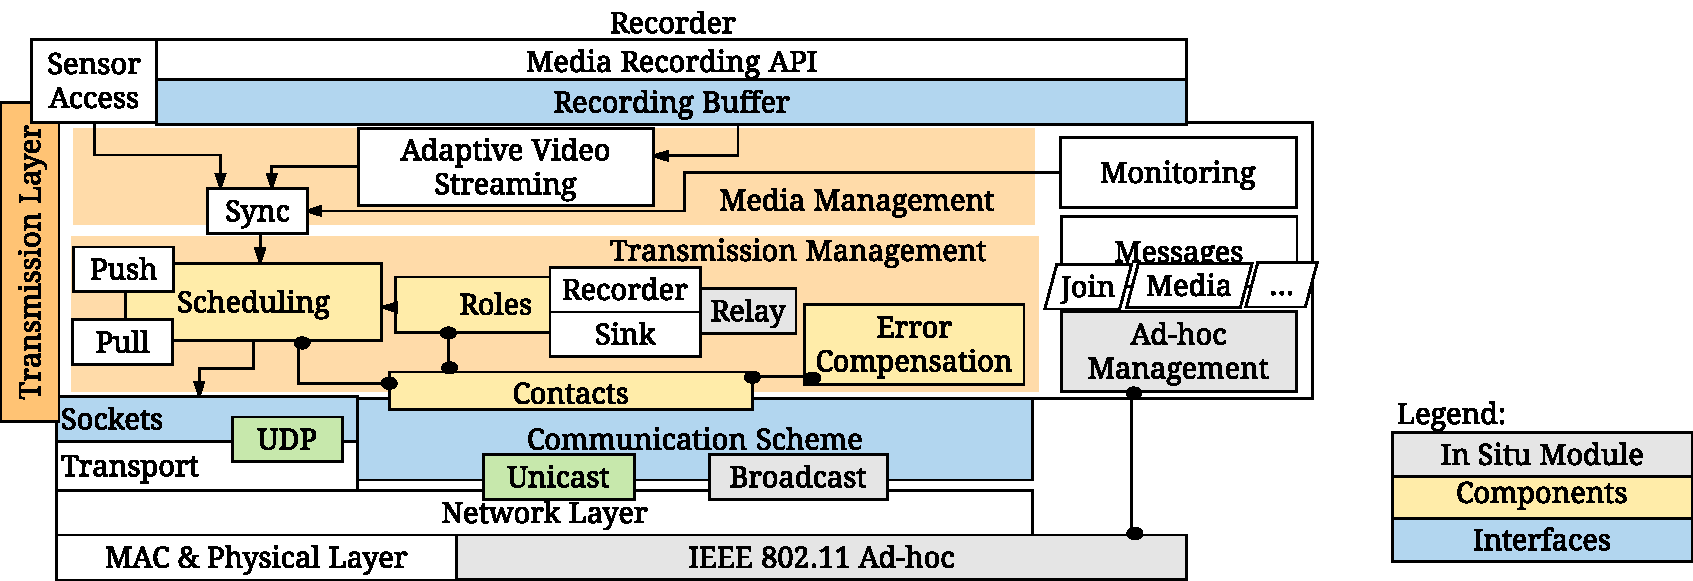
\includegraphics[width=\linewidth]{gfx/500_MobileUpload/architecture_liviu}
\caption[Architecture of \acf{LiViU}]{Architecture of LiViU for supporting remote and in situ streaming scenarios.}
\label{fig:522_architectureliviu}
\end{figure}

\subsection{Video Management}
On the recorder side, the media management is responsible for creating one or more valid media streams.
\subsubsection{Audio-Visual Streaming}
\ac{LiViU} understands media streams as audio-visual data, which are recorded from a recording device's internal sensors, i.e., cameras and microphones. The media streams are delivered in either a single media container or in two media containers independent of each other.
The media container encapsulates the media tracks and ensures that the receiver can initiate the video stream playback and an in-order consumption of the video stream.
As the visual part of the media stream constitutes a significantly higher portion of the generated data traffic, as well as the computational complexity, the focus for the remainder of this chapter lies solely on video - and thus, video streams.

To enable today's mobile recording devices to stream video in real-time, hardware implementations for compression are used\footnote{Supported hardware implementations for mobile devices are defined by the  \ac{OS}, as, e.g., for Android: https://developer.android.com/guide/appendix/media-formats.html; Visited on: 08/30/2016, or iOS: https://developer.apple.com/library/ios/technotes/tn2224; Visited on: 08/30/2016. }.
The support of hardware encoding capabilities allows for considering the H.264/\ac{AVC} encoding in this work.
The concepts can be mapped to the recently proposed H.265/\ac{HEVC}.
Both encoding standards rely on the encoding of a \ac{GoP}, which defines an independently decodable video chunk. 
Furthermore, as an abstraction from the network, the so-called \ac{NAL} units are used.
They encapsulate video segments, which can be streamed over a network, and independently interpreted by a decoder. % without any further information.
Receiving of a single \ac{NAL} unit does not mean that one or multiple video frames can be decoded, whereas a complete \ac{GoP} allows the same.
Thus, a \ac{GoP} usually consists of many \ac{NAL} units, when a video is being transmitted over a network.

A video receiving device needs meta information to setup a video decoder.
This metadata produced by the widely supported H.264/AVC codec includes the Sequence Parameter Set (\ac{NAL} unit type 7) and Picture Parameter Set (\ac{NAL} unit type 8).
The Sequence Parameter Set contains information to understand a sequence of encoded video frames, whereas the Picture Parameter Set defines parameters to understand how an individual frame can be decoded.
Both \ac{NAL} units parameterize the decoder on the receiver side of a stream to be able to decode a \ac{GoP} without any further information~\cite{ITU-TH2642016,ITU-TH2652015}.
This enables a receiver of a video stream to instantly play back or process the video stream - even if parts are lost.
\subsubsection{Adaptive Video Streaming}
\label{sec:522_adaptiveStreaming_LiViU}
Adaptive video streaming allows one to record from a single camera and encode the stream in different bit rate representations.
During a streaming session, the transmission component decides, what representation should be streamed depending on current network conditions.
Until now, this concept is solely available for the delivery of video streams and not on the recording device.
Industry solutions as well as research proposals~\cite{Seo2012} do not assume that it is feasible to create multiple representations to instantly switch between them.

This thesis discusses the extension of the media recording \ac{API} on Android phones to set up different encoding threads on the mobile device.
A realization is achieved, as the hardware encoding of current smartphone generations can be leveraged for the transcoding of video. 
Transcoding means the translation of video attributes (i.e., codec, frame rate, bit rate, resolution) from an incoming video stream to one or many output representations.
This is a computationally intensive process. 
The video codecs are set up with similar parameters but may differ in the target bit rate, frame rate, and video resolution.
Each received video frame is handed over to the video encoding thread.
As the sequential encoding of different resolutions and frame rates would be too time-consuming on the \ac{CPU}s of a smart mobile device, the graphics rendering \ac{API} of Android is used to run the transcoding on the \ac{GPU}.
Each raw video frame retrieved by the camera is converted into a two-dimensional texture, which is represented as a three-dimensional texture for multiple frames.
Using a texture, the \ac{GPU} on the mobile device allows quick manipulation of the resolution and frame rate.
The \ac{OpenGLES} library on the mobile devices is used\footnote{https://source.android.com/devices/graphics/arch-egl-opengl.html; Visited on: 09/23/2016}.
Each encoding thread operates on a copy of the texture and manipulates it according to the desired frame rate and resolution properties.
The final step hands the texture buffer to the respective video encoding object which leverages the built-in hardware to encode the representation at the desired bit rate.
The resulting H.264/\ac{AVC} raw video representations are consecutively written to the recording buffer in the main memory of a smart mobile device.

A real-time capable video parsing service analyzes the consecutively written video files and offers them to the transmission functionality of \ac{LiViU}. 
The complexity of understanding when a switch can be conducted without any artifacts on the receiver side is hidden in the parsing service.
This is possible, as the \ac{NAL} unit types 7 and 8 allow for determining the position of independently decodable video chunks.
Video chunk boundaries are determined by the \ac{GoP}.
These \ac{GoP}s can also be quickly identified while parsing the video stream using the \ac{NAL} unit of type 5 as they represent the start of a \ac{GoP}~\cite{ITU-TH2642016,ITU-TH2652015}.
The proposed approach transcodes a limited number of $N_{Rep}$ representations on the mobile devices during the streaming session in real-time ($N_{Rep}=4$ on an LG Nexus 5 with \ac{1080p}). 

\begin{figure}
\centering
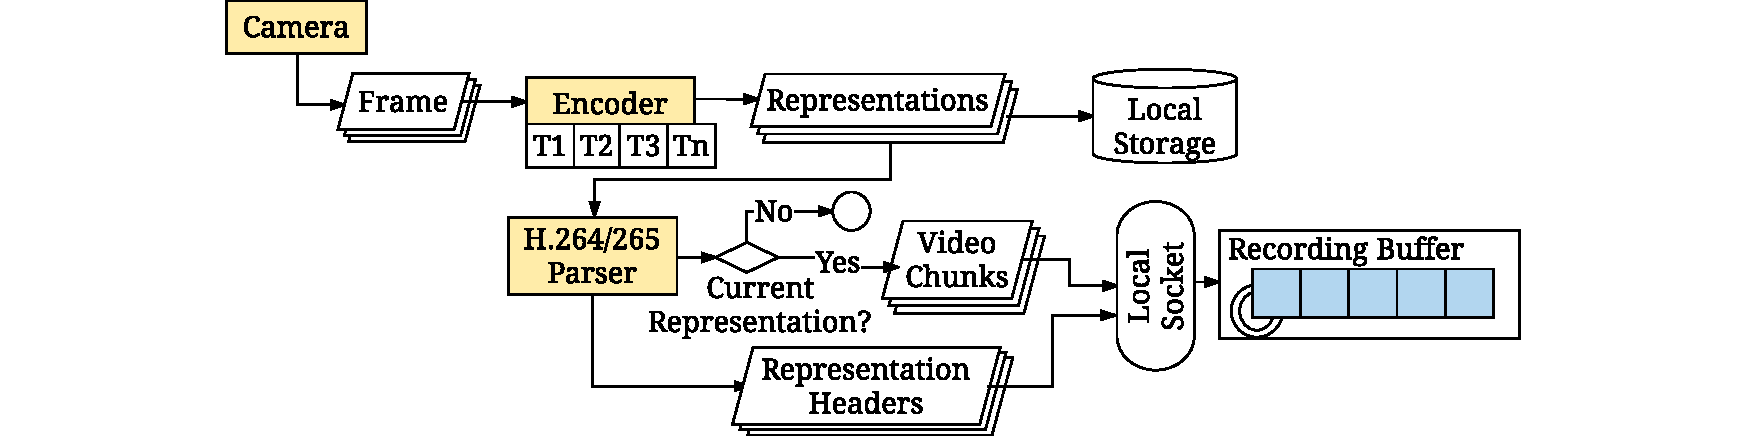
\includegraphics[width=\linewidth]{./gfx/500_MobileUpload/Video_Generation}
\caption{Generation of adaptive video streams on a smart mobile device.}
\label{fig:522_Video_Generation}
\end{figure}

Whereas video representations of different bit rates can be easily stitched, the frame rates and resolutions need a mapping by interpolating the dimensions to each other.
All resolutions that a mobile recorder generates need to be an integer multiple of the width and height of the lowest resolution.
Similarly, the frame rate needs to be an integer multiple of the lowest frame rate.
\subsubsection{Auxiliary Data}
Auxiliary data is required by many multimedia applications, especially for the video composition application discussed in Chapter~\ref{chapter:600_videocomposition}.
This data consists of monitoring data such as performance metrics (i.e., overhead, goodput, join time and latency) as well as auxiliary sensors.
Both describe environmental conditions when recording a video stream.

Auxiliary sensor readings are required for the quality assessment discussed in Chapter~\ref{chapter:550_scalable_quality_assessment}.
Sensors commonly in use are location providers such as the \ac{GPS}, accelerometer, gyroscope or the light sensor.

The data is stored in individual monitoring and sensor messages and transmitted independent of the video streams.
The scheduling of the respective messages can be defined by the application, but it ensures that readings are aggregated and sent at an adjustable frequency.
This frequency is chosen to address the requirements of the application, i.e., for just-in-time data processing, and should simultaneously reduce the overhead by sending as few messages as required.
All auxiliary data is annotated by timing information, which is required to link the reading to the respective video time.
\subsubsection{Synchronization of Streams}
To allow synchronization of the auxiliary data with the audio and video streams, \ac{NTP} is used.
It is assumed that all devices synchronize their clocks using central timing servers~\cite{rfc5905}. 
A constant Internet connection is assumed, which can then guarantee accuracy at an error of 10 milliseconds.
Synchronized clocks are used to annotate each message and each video chunk with timestamps to allow a resynchronization of video and auxiliary data streams. 
% -  -  -  -  -  -  -  -  -  -  -  -  -  -  -  - --
\subsection{Transmission}
\label{sec:522_Transmission}
Devices using \ac{LiViU} record video streams and upload them in a content-adaptive manner by using a reliable transmission layer.
This layer offers adaptive scheduling of video streams, coordination of the devices which generates a minimum of overhead, and capabilities to cope with the unreliability of \ac{UDP}.
Derived from the system model - proposed in Section~\ref{sec:520_extendedSystemModel} - the contact management module is integrated into \ac{LiViU}.
It runs on each device and allows remote devices to be represented as contacts: a combination of an \ac{IP} address and a port.
The contact types represent the roles of each device in a remote streaming scenario.
A device can either be a sender or a receiver of a video stream. 
\subsubsection{Message Scheduling}
\label{sec:522_message_scheduling}
The message scheduling can be classified into the quick stream joining procedure, scheduling type - either push or pull-based - and the timing of message sending. \paragraph{Push or Pull}
For different scenarios, a pull-based delivery is beneficial to cope with rapidly changing application needs.
\begin{figure}[tbh!]
\centering
\subfloat[Remote Upload]{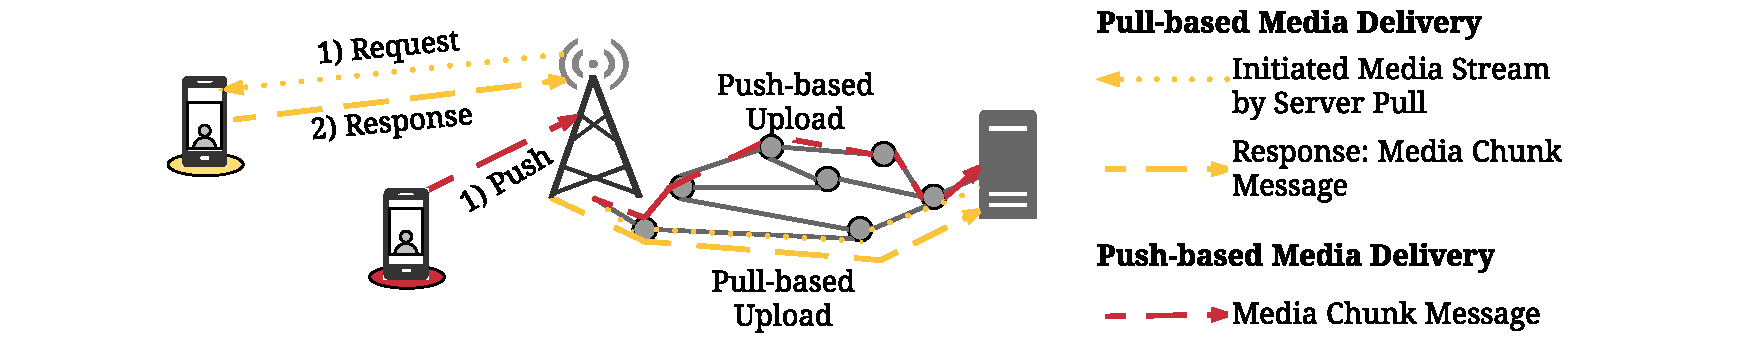
\includegraphics[width=\linewidth]{gfx/500_MobileUpload/Push_Pull_Schema_Remote}}\\
\subfloat[In Situ Upload]{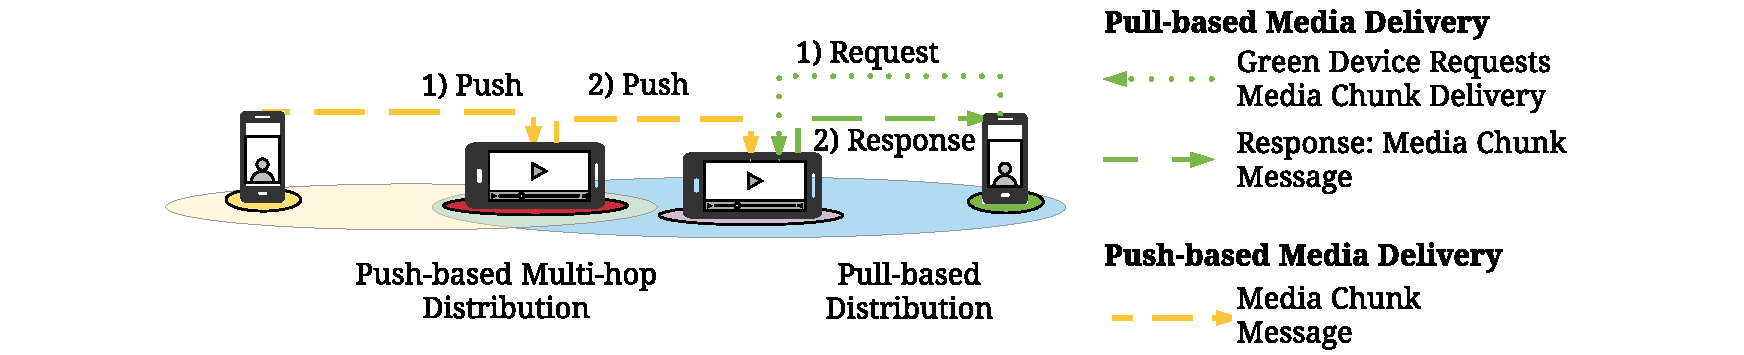
\includegraphics[width=\linewidth]{gfx/500_MobileUpload/Push_Pull_Schema_InSitu}}\\
\caption[Overview of different scheduling mechanisms]{Push and pull scheduling for uploading video streams in remote and in situ streaming sessions.}
\label{fig:522_pushpullschemaremote}
\end{figure}
\ac{LiViU} can adapt between different scheduling schemes: push-based delivery of media messages and pull-based retrieval of the same (see Figure~\ref{fig:522_pushpullschemaremote}).
By default, \ac{LiViU} uses a push-based delivery to allow a low-delay streaming at a minimal overhead.
The switch between two modes can be initiated by a "Pause Request Message" sent by the receiver of a media stream, which indicates that the default mode - push-based - is stopped.
This message includes a hint to reply to the request.
As soon as the request is acknowledged by the media recorder, the media receiver requests subsequent media chunks.
The pull-based delivery of chunks is controlled by the application on the receiver side, which can determine when to request the appropriate media chunk.
\paragraph{Quick Stream Joining Procedure}
By default, a push-based delivery is chosen, which allows a minimal join time.
Existing protocols rely on long-lasting join procedures and thus increase the join time.
\ac{LiViU} applies quick streaming by assuming that a session can be successfully established without an initial handshake procedure.
The join procedure is not executed in a first step; instead, the recording device assumes, that the remote end can be reached, and instantly starts recording and sending video chunks.
By using \ac{UDP}, a connection-establishing procedure as known from \ac{TCP} is avoided.
As the network conditions are initially unknown, the minimal representation is chosen to be streamed to achieve the highest likelihood of timely video stream processing on the receiver side.

The joining procedure is still required to establish a reliable connection state, and to coordinate desired streaming properties such as the resolution frame rate and desired bit rate, as well as encryption or \ac{DRM} mechanisms.
This is achieved as the join procedure is initiated after the first video chunk is transmitted.
As no reliable throughput measurements are available before the streaming begins and to avoid congestion, the join procedure is not executed in parallel to the video transmission, but slightly delayed.
\paragraph{Timing}
The push-based delivery enables \ac{LiViU} to instantly hand over messages provided by the media recording \ac{API} to lower communication layers.

Two exceptions exist for timing video and "leave" messages. 
Once a mobile recorder indicates that it is time to stop streaming, the "leave" message transmission is postponed until the remaining video chunks are transmitted. 
The leave message indicates that the video sinks on the receiver's side can be closed, and no more video chunks will be sent.

Timing of video messages can be adjusted by a request on the receiver side to either continue or pause the transmission.
This indicates to \ac{LiViU} to switch to a pull-based delivery scheme.
Here, the multimedia application on the receiver side determines when to request a video chunk, e.g., requesting only every $n$-th video chunk.
Video chunks contain segments that can be independently decoded; this allows for a video quality assessment of parts of a stream (as proposed in Chapter~\ref{chapter:550_scalable_quality_assessment}) and needed by a video composition system (as proposed in Chapter~\ref{chapter:600_videocomposition}).
\subsubsection{Messages}
\ac{LiViU} is a message-oriented media streaming protocol.
Each message consists of a header and a body element.
The body contains the payload, which is specific to the message type but can be empty.
The header is used by the \ac{LiViU} protocol to steer the protocol and enable routing on the lower layers (see Figure~\ref{fig:522_messageformat}).
Each header is designed to generate the least possible overhead, which is also the reason why the headers differ in remote streaming and "in situ streaming".

\begin{figure}
\centering
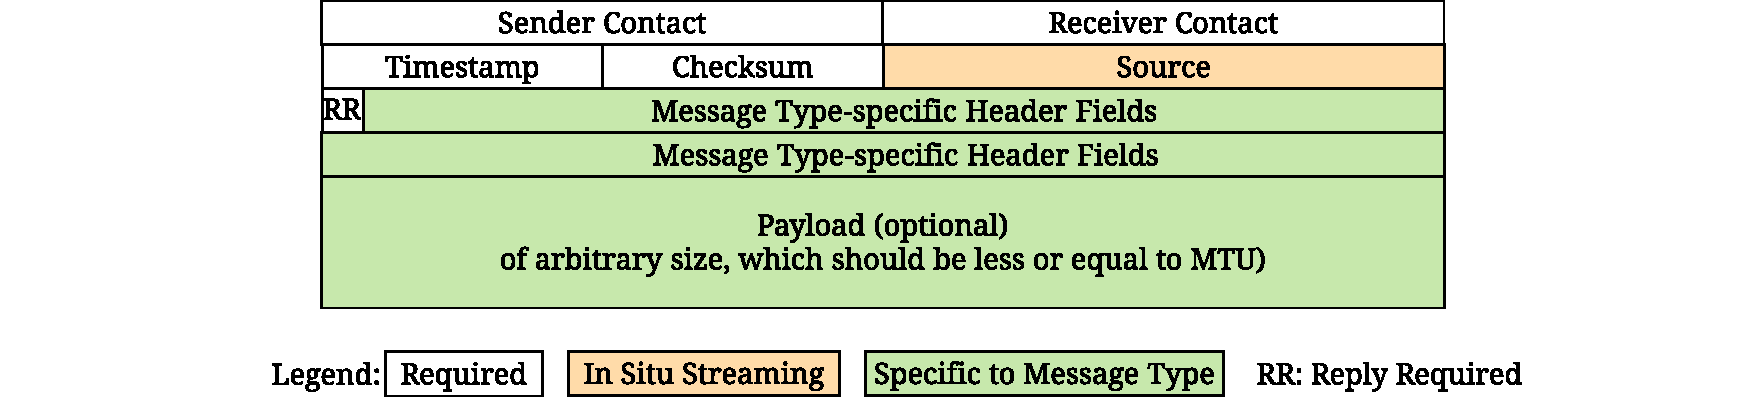
\includegraphics[width=\linewidth]{gfx/500_MobileUpload/Message_Format}
\caption{Format of a LiViU message including header fields.}
\label{fig:522_messageformat}
\end{figure}

The header of each message consists of at least the sender and receiver contact information. 
Each \ac{LiViU} header can also have a notification if a reply is required, and a timestamp that represents the message creation time. 
Whereas the sender and receiver contact information are required for communication, the timestamp and reply requests are specific to the \ac{LiViU} protocol. 
As the protocol overhead shall be kept low, not all messages are acknowledged automatically. 
Not discussed further is a \ac{CRC} checksum which indicates the validity of each message.
Additional header fields are available depending on the message type.
The different message types for a remote streaming session are described below.
\paragraph{Join Message}
A join message indicates to a video stream receiver that a new streaming session begins. 
Usually, it is received after the server already received some video chunks due to the integrated quick stream protocol.
A join message includes the video information that is transmitted including the representation descriptions, i.e., number of representations, their frame rates, resolutions, and bit rates\footnote{When a server receives the first video chunk, it does not have to know the video encoding used as it can parse the initial bytes of a video stream.}.
Also, a list of available auxiliary sensors is added.
Once processed by the receiver, a reply is sent to the sender of the join message to acknowledge that the streaming session is completely established. 
\paragraph{Leave Message}
The leave message indicates that all media files related to a recorder can be closed and state information established on the receiver side associated with the recorder can be deleted.
After the leave message is received and processed, no further messages from  this sender can be processed.

\paragraph{Media Message}
The main purpose of \ac{LiViU} is to transmit video and audio streams to remote receivers.
Media messages contain chunks of the media as a payload, with variable sizes. As metadata, these messages contain header information on the streamed representation, the current chunk identifier, and the media type. The representation information is a single integer indicating the representation index. The chunk identifier is unique per device and media type. It is an increasing integer, which indicates the sequence of a media stream. The type of message indicates whether the current stream consists of an audio or video container. Media messages additionally contain information on the latest chunk available on the recorder side to allow a receiver to estimate the delay.

\paragraph{Auxiliary Data Message}
Auxiliary data messages consist of sensor messages and monitoring messages. Only the auxiliary sensor messages are explained here. 
As auxiliary sensor data is comparably small, if possible multiple samples from a sensor are packed into a single message for transmission. 
The timestamps indicate when the sensor generated those samples. 
A type flag indicates what sensor produced the sample. 
The typical sensors used by multimedia applications are location providers, e.g., the \ac{GPS}, gyroscope, accelerometer and light sensor.
\paragraph{Pause and Record Messages}
Devices that are recording a video can decide to stop streaming video to a remote receiver, e.g. if the network conditions are too poor to stream the lowest representation.
Pause and record messages allow the client to coordinate to actively use or stop \ac{LiViU}.
Pausing the \ac{MBS} indicates that no additional messages are sent until a record message is received again.
This temporarily disables the scheduling, but keeps track of active contacts.
A pause message is necessary if the push-based delivery of a video shall be replaced by a pull-based receiver side retrieval of video.
These messages contain no additional header fields.

\paragraph{Request Message}
As \ac{LiViU} can operate in both pull- and push-based scheduling, it allows the receiver to request all video chunks individually.
Also, the coordination messages - except for join and leave - can be requested.
Thus, in pull-based scheduling, the receiver of a media stream would regularly send request messages containing the chunk identifier and a reply request to the recording device.
The receiving device determines the rate in which video chunks are requested. Request messages contain the same header fields as the respective message type being requested.

Some special forms of requests are available for controlling the \ac{LiViU} scheduling. 
Rate control requests are introduced for video streams to determine at what intervals chunks will be pushed, and which representation index is used. 
% -  -  -  -  -  -  -  -  -  -  -  -  - --
\subsubsection{Coping with the Unreliability of UDP}
\label{sec:522_CopingUnreliabilityUDP}
\ac{UDP} is unreliable regarding congestion avoidance, in-order message delivery and packet losses or payload errors.
Whereas the avoidance of congestion is out of the scope of this work, our focus lies on the in-order processing and compensation of packet losses.
It is assumed that payload errors can easily be detected by a checksum (\ac{CRC}) transmitted with the message.

The loss of a message can be compensated by encoding the content in a redundant manner in the remaining messages, as, e.g., proposed by \ac{FEC}, or by solving the problem using a re-request of the messages in a manner as proposed by \ac{ARQ}.
In \ac{ARQ}, packet losses or errors in messages, e.g., detected via \ac{CRC}, are compensated using a retransmission of the messages.
Also, it ensures in-order processing, as a sliding window is assumed on both the sender and receiver side of messages, which annotates individual messages by a sequence number.
Thus, \ac{ARQ} assumes a duplex channel for communication.

The realization of a selective repeat mechanism for \ac{LiViU} uses a sliding window on the sender and receiver side. 
If a message is found that is not received in the correct order - or that is erroneous - subsequent messages are buffered. 
A negative acknowledgment (request message) is sent to the sender to request the missing video chunk. 
As soon the message is received correctly, the subsequent, buffered messages are also processed. 
\begin{figure}
	\centering
	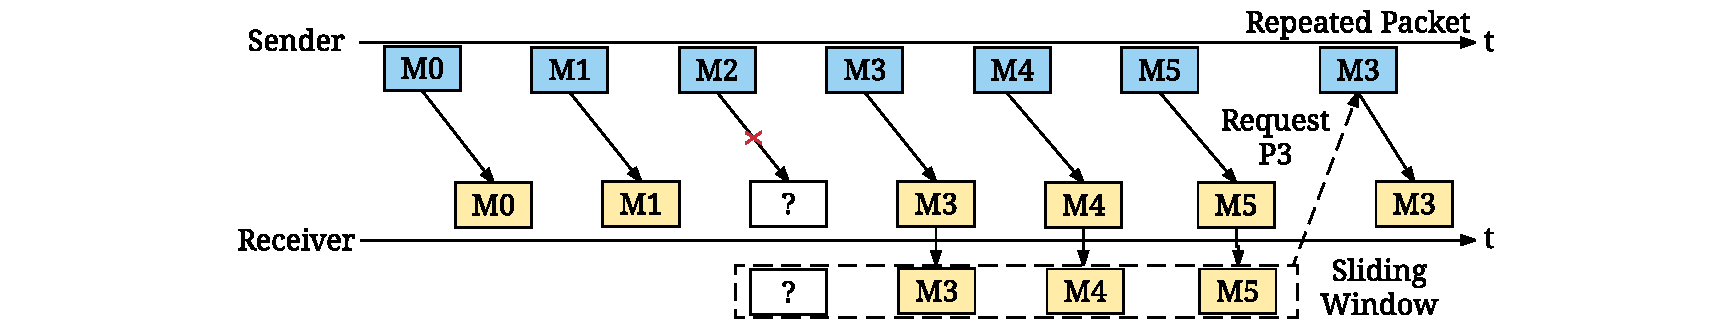
\includegraphics[width=\linewidth]{./gfx/500_MobileUpload/Sliding_Window_Selective_repeat}
	\caption[Request-repeat ARQ scheme]{The proposed method for compensating transmission errors using unreliable UDP connection: a request-repeat ARQ scheme.}
	\label{fig:522_slidingwindowselectiverepeat}
\end{figure}

Figure~\ref{fig:522_slidingwindowselectiverepeat} depicts the sliding window which can store $M$ packets on the receiver and sender side.
The order of the messages is not guaranteed by \ac{UDP}, so the sliding window reestablishes the order and detects if packets in a sequence are missing or if a message is corrupt.
In contrast to other selective repeat implementations, no messages are acknowledged.
Only missing or corrupted messages are requested again from the sender.
The correctness of a message is validated using the \ac{CRC}.
Missing packets are identified by the sequence numbers created while recording.
If a media chunk message with an index $> i$ is received but $i$ is missing, a singleton deadline timer of $D_t+2\times \sigma D_t$ is set, after which the chunk is requested, assuming a normal distribution of the delay.
$D_t$ represents the last sampled end-to-end delay measurement.
This approach ensures a reliable delivery of messages and an in-time and in-order processing of messages.
A detected error is compensated similarly to a packet loss by requesting the message again.
\subsubsection{Goodput-related Media Adaptation}
The link between transmission functionality and the media management is the video representation adaptation based on the current throughput measurements.
From the metrics defined in Section~\ref{sec:520_metrics}, the current application layer throughput is derived.
It is used for deciding which video representation to choose, and is thus calculated each time a video adaptation can be executed.
Bit rates of the representations are compared with the current throughput, and the representation index ($id_{R}$) is chosen whose bit rate is equal or slightly below the current throughput:
\begin{equation}
\label{optQual:formula1}
argmax(B(id_{R})) \quad\quad where\quad B(id_{R}) \leq TP_t
\end{equation}
 where $B()$ represents the bit rate of representation $id_{R}$.
 It is assumed that a higher identifier indicates a higher bit rate.
$TP_t$ represents the throughput measured at time $t$.
Independent of the throughput, a multimedia application, e.g., for video composition, can request to deliver a specific representation.
\subsubsection{Monitoring}
The transmission layer, especially the media adaptation, requires a continuous and reliable measurement of the end-to-end throughput and delay.
An independent monitoring service conducting active throughput measurements is chosen, as proposed by Stohr et al.~\cite{Stohr2014,Stohr2016}.
The monitoring service has been modeled, designed and evaluated using \ac{LiViU} but is not in the focus of this work.
